\documentclass[10pt]{article}
\usepackage[polish]{babel}
\usepackage[utf8]{inputenc}
\usepackage[T1]{fontenc}
\usepackage{graphicx}
\usepackage[export]{adjustbox}
\graphicspath{ {./images/} }
\usepackage{amsmath}
\usepackage{amsfonts}
\usepackage{amssymb}
\usepackage[version=4]{mhchem}
\usepackage{stmaryrd}
\usepackage{multirow}

\title{CENTRALNA }

\author{}
\date{}


\begin{document}
\maketitle
KOMISJA\\
EGZAMINACYJNA\\
Arkusz zawiera informacje prawnie chronione do momentu rozpoczęcia egzaminu.

UZUPELNIA ZDAJĄCY

KOD\\
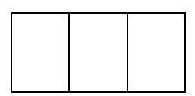
\includegraphics[max width=\textwidth, center]{2024_11_21_d51d653f4fe4a5bb0c33g-01}

PESEL\\
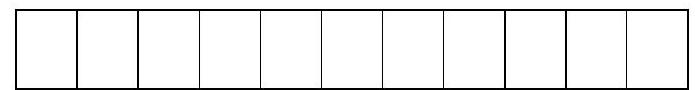
\includegraphics[max width=\textwidth, center]{2024_11_21_d51d653f4fe4a5bb0c33g-01(1)}

\begin{center}
\begin{tabular}{c}
 \\
miejsce \\
na naklejke \\
 \\
\hline
\end{tabular}
\end{center}

\section*{EGZAMIN MATURALNY}
\section*{Z MATEMATYKI}
\section*{POZIOM PODSTAWOWY}
\section*{Instrukcja dla zdającego}
\begin{enumerate}
  \item Sprawdź, czy arkusz egzaminacyjny zawiera 26 stron (zadania 1-34). Ewentualny brak zgłoś przewodniczącemu zespołu nadzorującego egzamin.
  \item Rozwiązania zadań i odpowiedzi wpisuj w miejscu na to przeznaczonym.
  \item Odpowiedzi do zadań zamkniętych (1-25) zaznacz na karcie odpowiedzi, w części karty przeznaczonej dla zdającego. Zamaluj \(\square\) pola do tego przeznaczone. Błędne zaznaczenie otocz kółkiem ( i zaznacz właściwe.
  \item Pamiętaj, że pominięcie argumentacji lub istotnych obliczeń w rozwiązaniu zadania otwartego (26-34) może spowodować, że za to rozwiązanie nie otrzymasz pełnej liczby punktów.
  \item Pisz czytelnie i używaj tylko długopisu lub pióra z czarnym tuszem lub atramentem.
  \item Nie używaj korektora, a błędne zapisy wyraźnie przekreśl.
  \item Pamiętaj, że zapisy w brudnopisie nie będą oceniane.
  \item Możesz korzystać z zestawu wzorów matematycznych, cyrkla i linijki oraz kalkulatora prostego.
  \item Na tej stronie oraz na karcie odpowiedzi wpisz swój numer PESEL i przyklej naklejkę z kodem.
  \item Nie wpisuj żadnych znaków w części przeznaczonej dla egzaminatora.
\end{enumerate}

7 MAJA 2019\\
UZUPELNIA ZESPÓŁ NADZORUJĄCY\\
Uprawnienia zdającego do:\\

\includegraphics[max width=\textwidth, center]{2024_11_21_d51d653f4fe4a5bb0c33g-01(2)}\\
dostosowania kryteriów oceniania\\
nieprzenoszenia zaznaczeń na kartę\\
\(\square\) dostosowania\\
w zw. z dyskalkulią

Godzina rozpoczęcia:\\
9:00

Czas pracy:\\
170 minut

Liczba punktów\\
do uzyskania: 50

MMA-P1\_1P-192

\section*{ZADANIA ZAMKNIĘTE}
W każdym z zadań od 1. do 25. wybierz izaznacz na karcie odpowiedzi poprawną odpowiedź.

\section*{Zadanie 1. (1 pht)}
Liczba \(\log _{\sqrt{2}} 2\) jest równa\\
A. 2\\
B. 4\\
C. \(\sqrt{2}\)\\
D. \(\frac{1}{2}\)

\section*{Zadanie 2. (1 pht)}
Liczba naturalna \(n=2^{14} \cdot 5^{15} \mathrm{w}\) zapisie dziesiętnym ma\\
A. 14 cyfr\\
B. 15 cyfr\\
C. 16 cyfr\\
D. 30 cyfr

\section*{Zadanie 3. (1 pht)}
W pewnym banku prowizja od udzielanych kredytów hipotecznych przez cały styczeń była równa \(4 \%\). Na początku lutego ten bank obniżył wysokość prowizji od wszystkich kredytów o 1 punkt procentowy. Oznacza to, że prowizja od kredytów hipotecznych w tym banku zmniejszyła sięo\\
A. \(1 \%\)\\
B. \(25 \%\)\\
C. \(33 \%\)\\
D. \(75 \%\)

\section*{Zadanie 4. (1 pht)}
Równość \(\frac{1}{4}+\frac{1}{5}+\frac{1}{a}=1\) jest prawdziwa dla\\
A. \(a=\frac{11}{20}\)\\
B. \(a=\frac{8}{9}\)\\
C. \(a=\frac{9}{8}\)\\
D. \(a=\frac{20}{11}\)

\section*{Zadanie 5. (1 pkt)}
Para liczb \(x=2\) i \(y=2\) jest rozwiązaniem układu równań \(\left\{\begin{array}{c}a x+y=4 \\ -2 x+3 y=2 a\end{array}\right.\) dla\\
A. \(a=-1\)\\
B. \(a=1\)\\
C. \(a=-2\)\\
D. \(a=2\)

\section*{Zadanie 6. (1 pkt)}
Równanie \(\frac{(x-1)(x+2)}{x-3}=0\)\\
A. ma trzy różne rozwiązania: \(x=1, x=3, x=-2\).\\
B. ma trzy różne rozwiązania: \(x=-1, x=-3, x=2\).\\
C. ma dwa różne rozwiązania: \(x=1, x=-2\).\\
D. ma dwa różne rozwiązania: \(x=-1, x=2\).

\section*{BRUDNOPIS (nie podlega ocenie)}
\begin{center}

\includegraphics[max width=\textwidth]{2024_11_21_d51d653f4fe4a5bb0c33g-03}
\end{center}

\section*{Zadanie 7. (1 pkt)}
Miejscem zerowym funkcji liniowej \(f\) określonej wzorem \(f(x)=3(x+1)-6 \sqrt{3}\) jest liczba\\
A. \(3-6 \sqrt{3}\)\\
B. \(1-6 \sqrt{3}\)\\
C. \(2 \sqrt{3}-1\)\\
D. \(2 \sqrt{3}-\frac{1}{3}\)

\section*{Informacja do zadań 8.-10.}
Na rysunku przedstawiony jest fragment paraboli będącej wykresem funkcji kwadratowej \(f\). Wierzchołkiem tej paraboli jest punkt \(W=(2,-4)\). Liczby 0 i 4 to miejsca zerowe funkcji \(f\).\\
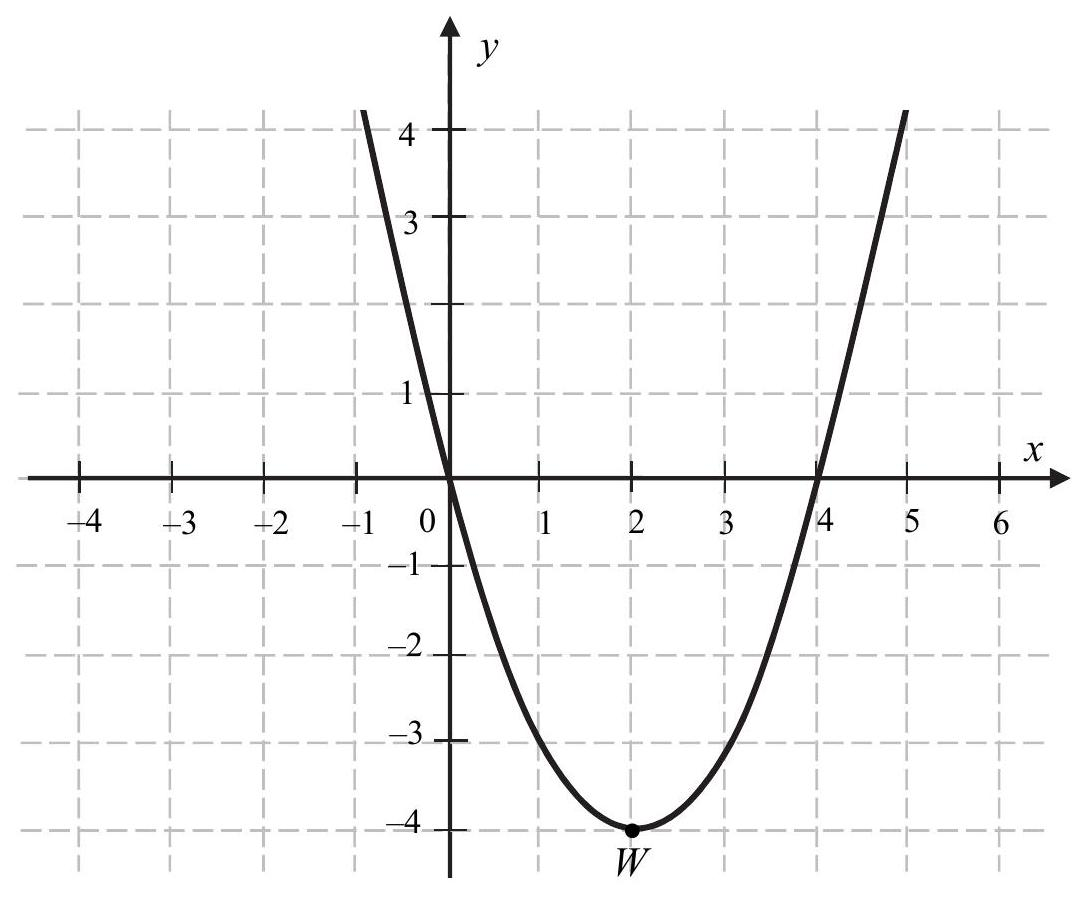
\includegraphics[max width=\textwidth, center]{2024_11_21_d51d653f4fe4a5bb0c33g-04}

\section*{Zadanie 8. (1 pht)}
Zbiorem wartości funkcji \(f\) jest przedział\\
A. \((-\infty, 0\rangle\)\\
B. \(\langle 0,4\rangle\)\\
C. \((-4,+\infty)\)\\
D. \((4,+\infty)\)

\section*{Zadanie 9. (1 pkt)}
Największa wartość funkcji \(f\) w przedziale \(\langle 1,4\rangle\) jest równa\\
A. -3\\
B. -4\\
C. 4\\
D. 0

\section*{Zadanie 10. (1 pkt)}
Osią symetrii wykresu funkcji \(f\) jest prosta o równaniu\\
A. \(y=-4\)\\
B. \(x=-4\)\\
C. \(y=2\)\\
D. \(x=2\)

\section*{BRUDNOPIS (nie podlega ocenie)}
\begin{center}

\includegraphics[max width=\textwidth]{2024_11_21_d51d653f4fe4a5bb0c33g-05}
\end{center}

\section*{Zadanie 11. (1 pkt)}
W ciągu arytmetycznym \(\left(a_{n}\right)\), określonym dla \(n \geq 1\), dane są dwa wyrazy: \(a_{1}=7\) i \(a_{8}=-49\). Suma ośmiu początkowych wyrazów tego ciągu jest równa\\
A. -168\\
B. -189\\
C. -21\\
D. -42

\section*{Zadanie 12. (1 pkt)}
Dany jest ciąg geometryczny \(\left(a_{n}\right)\), określony dla \(n \geq 1\). Wszystkie wyrazy tego ciągu są dodatnie i spełniony jest warunek \(\frac{a_{5}}{a_{3}}=\frac{1}{9}\). Iloraz tego ciągu jest równy\\
A. \(\frac{1}{3}\)\\
B. \(\frac{1}{\sqrt{3}}\)\\
C. 3\\
D. \(\sqrt{3}\)

\section*{Zadanie 13. (1 pkt)}
Sinus kąta ostrego \(\alpha\) jest równy \(\frac{4}{5}\). Wtedy\\
A. \(\cos \alpha=\frac{5}{4}\)\\
B. \(\cos \alpha=\frac{1}{5}\)\\
C. \(\cos \alpha=\frac{9}{25}\)\\
D. \(\cos \alpha=\frac{3}{5}\)

\section*{Zadanie 14. (1 pkt)}
Punkty \(D\) i \(E\) leżą na okręgu opisanym na trójkącie równobocznym \(A B C\) (zobacz rysunek). Odcinek \(C D\) jest średnicą tego okręgu. Kąt wpisany \(D E B\) ma miarę \(\alpha\).\\
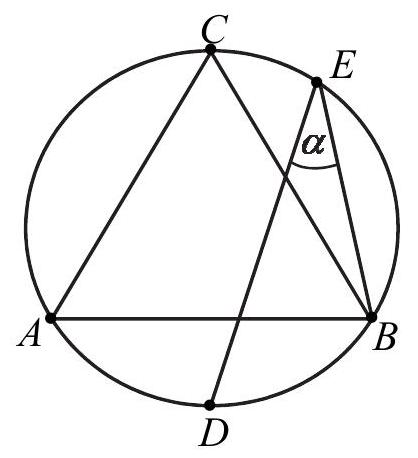
\includegraphics[max width=\textwidth, center]{2024_11_21_d51d653f4fe4a5bb0c33g-06}

\section*{Zatem}
A. \(\alpha=30^{\circ}\)\\
B. \(\alpha<30^{\circ}\)\\
C. \(\alpha>45^{\circ}\)\\
D. \(\alpha=45^{\circ}\)

\section*{BRUDNOPIS (nie podlega ocenie)}
\begin{center}

\includegraphics[max width=\textwidth]{2024_11_21_d51d653f4fe4a5bb0c33g-07}
\end{center}

\section*{Zadanie 15. (1 pkt)}
Dane są dwa okręgi: okrąg o środku w punkcie \(O\) i promieniu 5 oraz okrąg o środku w punkcie \(P\) i promieniu 3. Odcinek \(O P\) ma długość 16. Prosta \(A B\) jest styczna do tych okręgów w punktach \(A\) i \(B\). Ponadto prosta \(A B\) przecina odcinek \(O P\) w punkcie \(K\) (zobacz rysunek).\\
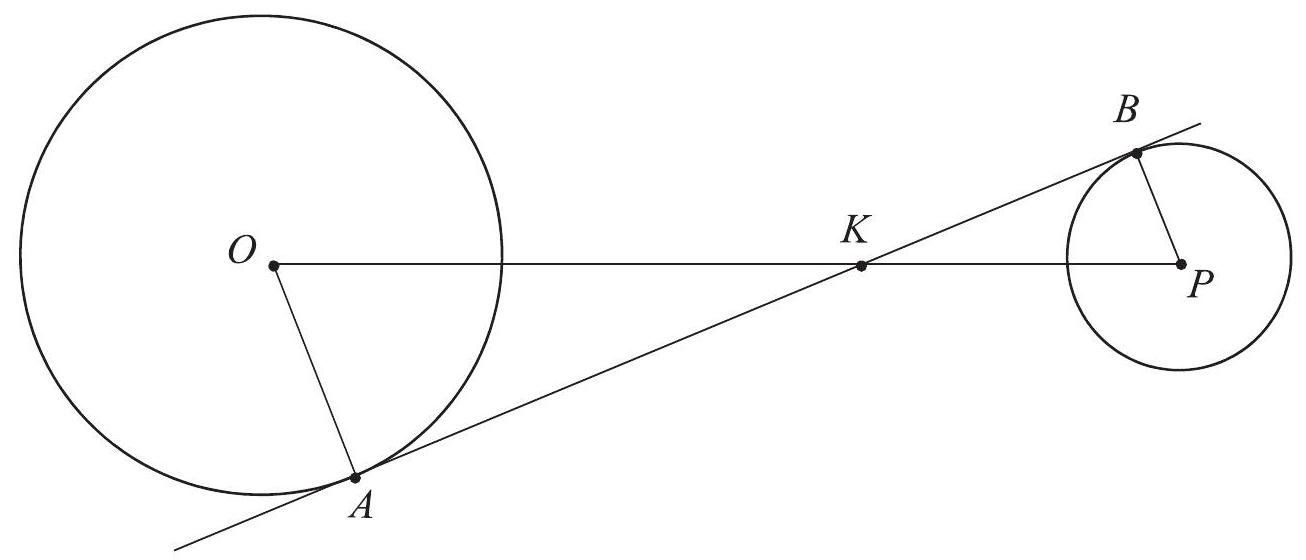
\includegraphics[max width=\textwidth, center]{2024_11_21_d51d653f4fe4a5bb0c33g-08}

Wtedy\\
A. \(|O K|=6\)\\
B. \(|O K|=8\)\\
C. \(|O K|=10\)\\
D. \(|O K|=12\)

\section*{Zadanie 16. (1 pkt)}
Dany jest romb o boku długości 4 i kącie rozwartym \(150^{\circ}\). Pole tego rombu jest równe\\
A. 8\\
B. 12\\
C. \(8 \sqrt{3}\)\\
D. 16

\section*{Zadanie 17. (1 pkt)}
Proste o równaniach \(y=(2 m+2) x-2019\) oraz \(y=(3 m-3) x+2019\) są równoległe, gdy\\
A. \(m=-1\)\\
B. \(m=0\)\\
C. \(m=1\)\\
D. \(m=5\)

\section*{Zadanie 18. (1 pkt)}
Prosta o równaniu \(y=a x+b\) jest prostopadła do prostej o równaniu \(y=-4 x+1\) i przechodzi przez punkt \(P=\left(\frac{1}{2}, 0\right)\), gdy\\
A. \(a=-4\) i \(b=-2\)\\
B. \(\quad a=\frac{1}{4}\) i \(b=-\frac{1}{8}\)\\
C. \(a=-4\) i \(b=2\)\\
D. \(a=\frac{1}{4} \mathrm{i} b=\frac{1}{2}\)

\section*{BRUDNOPIS (nie podlega ocenie)}
\begin{center}

\includegraphics[max width=\textwidth]{2024_11_21_d51d653f4fe4a5bb0c33g-09}
\end{center}

\section*{Zadanie 19. (1 pkt)}
Na rysunku przedstawiony jest fragment wykresu funkcji liniowej \(f\). Na wykresie tej funkcji leżą punkty \(A=(0,4)\) i \(B=(2,2)\).\\
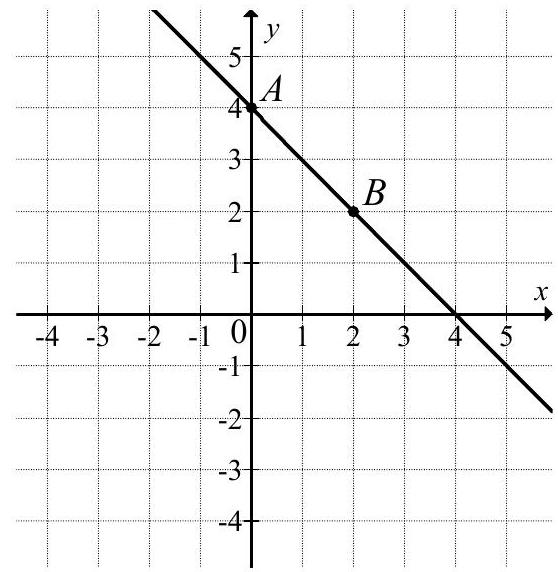
\includegraphics[max width=\textwidth, center]{2024_11_21_d51d653f4fe4a5bb0c33g-10}

Obrazem prostej \(A B\) w symetrii względem początku układu współrzędnych jest wykres funkcji \(g\) określonej wzorem\\
A. \(g(x)=x+4\)\\
B. \(g(x)=x-4\)\\
C. \(g(x)=-x-4\)\\
D. \(g(x)=-x+4\)

\section*{Zadanie 20. (1 pkt)}
Dane są punkty o współrzędnych \(A=(-2,5)\) oraz \(B=(4,-1)\). Średnica okręgu wpisanego w kwadrat o boku \(A B\) jest równa\\
A. 12\\
B. 6\\
C. \(6 \sqrt{2}\)\\
D. \(2 \sqrt{6}\)

\section*{Zadanie 21. (1 pkt)}
Promień \(A S\) podstawy walca jest równy połowie wysokości \(O S\) tego walca. Sinus kąta \(O A S\) (zobacz rysunek) jest równy\\
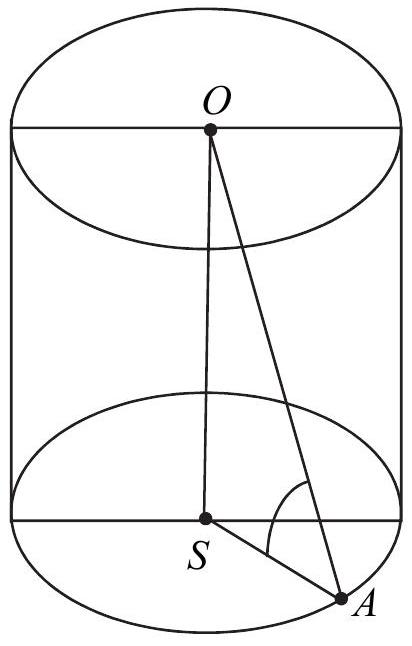
\includegraphics[max width=\textwidth, center]{2024_11_21_d51d653f4fe4a5bb0c33g-10(1)}\\
A. \(\frac{\sqrt{5}}{2}\)\\
B. \(\frac{2 \sqrt{5}}{5}\)\\
C. \(\frac{1}{2}\)\\
D. 1

\section*{BRUDNOPIS (nie podlega ocenie)}
\begin{center}

\includegraphics[max width=\textwidth]{2024_11_21_d51d653f4fe4a5bb0c33g-11}
\end{center}

\section*{Zadanie 22. (1 pkt)}
Podstawą ostrosłupa prawidłowego czworokątnego \(A B C D S\) jest kwadrat \(A B C D\). Wszystkie ściany boczne tego ostrosłupa są trójkątami równobocznymi.\\
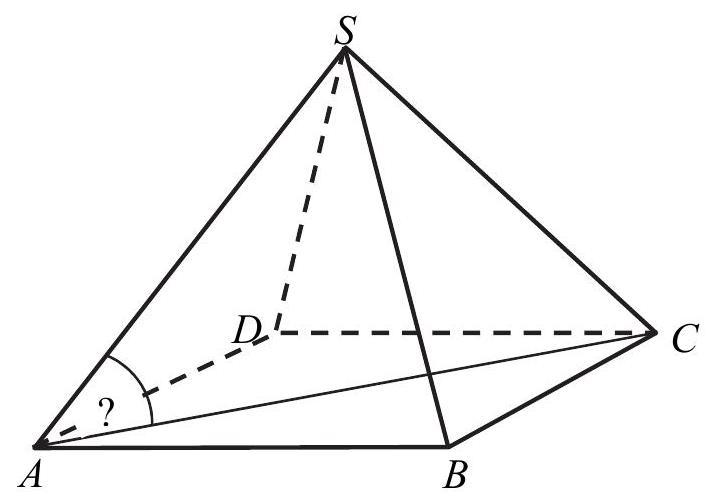
\includegraphics[max width=\textwidth, center]{2024_11_21_d51d653f4fe4a5bb0c33g-12}

Miara kąta \(S A C\) jest równa\\
A. \(90^{\circ}\)\\
B. \(75^{\circ}\)\\
C. \(60^{\circ}\)\\
D. \(45^{\circ}\)

\section*{Zadanie 23. (1 pkt)}
Mediana zestawu sześciu danych liczb: \(4,8,21, a, 16,25\), jest równa 14. Zatem\\
A. \(a=7\)\\
B. \(a=12\)\\
C. \(a=14\)\\
D. \(a=20\)

\section*{Zadanie 24. (1 pkt)}
Wszystkich liczb pięciocyfrowych, w których występują wyłącznie cyfry 0, 2, 5, jest\\
A. 12\\
B. 36\\
C. 162\\
D. 243

\section*{Zadanie 25. (1 pkt)}
W pudełku jest 40 kul. Wśród nich jest 35 kul białych, a pozostałe to kule czerwone. Prawdopodobieństwo wylosowania każdej kuli jest takie samo. Z pudełka losujemy jedną kulę. Prawdopodobieństwo zdarzenia polegającego na tym, że otrzymamy kulę czerwoną, jest równe\\
A. \(\frac{1}{8}\)\\
B. \(\frac{1}{5}\)\\
C. \(\frac{1}{40}\)\\
D. \(\frac{1}{35}\)

\section*{BRUDNOPIS (nie podlega ocenie)}
\begin{center}

\includegraphics[max width=\textwidth]{2024_11_21_d51d653f4fe4a5bb0c33g-13}
\end{center}

\section*{Zadanie 26. (2 pkt)}
Rozwiąż równanie \(x^{3}-5 x^{2}-9 x+45=0\).\\

\includegraphics[max width=\textwidth, center]{2024_11_21_d51d653f4fe4a5bb0c33g-14}\\
\(\qquad\)

\section*{Zadanie 27. (2 pkt)}
Rozwiąż nierówność \(3 x^{2}-16 x+16>0\).

\begin{center}
\begin{tabular}{|c|c|c|c|c|c|c|c|c|c|c|c|c|c|c|c|c|c|c|c|c|c|c|c|c|c|c|}
\hline
 &  &  &  &  &  &  &  &  &  &  &  &  &  &  &  &  &  &  &  &  &  &  &  &  &  &  \\
\hline
 &  &  &  &  &  &  &  &  &  &  &  &  &  &  &  &  &  &  &  &  &  &  &  &  &  &  \\
\hline
 &  &  &  &  &  &  &  &  &  &  &  &  &  &  &  &  &  &  &  &  &  &  &  &  &  &  \\
\hline
 &  &  &  &  &  &  &  &  &  &  &  &  &  &  &  &  &  &  &  &  &  &  &  &  &  &  \\
\hline
 &  &  &  &  &  &  &  &  &  &  &  &  &  &  &  &  &  &  &  &  &  &  &  &  &  &  \\
\hline
 &  &  &  &  &  &  &  &  &  &  &  &  &  &  &  &  &  &  &  &  &  &  &  &  &  &  \\
\hline
 &  &  &  &  &  &  &  &  &  &  &  &  &  &  &  &  &  &  &  &  &  &  &  &  &  &  \\
\hline
 &  &  &  &  &  &  &  &  &  &  &  &  &  &  &  &  &  &  &  &  &  &  &  &  &  &  \\
\hline
 &  &  &  &  &  &  &  &  &  &  &  &  &  &  &  &  &  &  &  &  &  &  &  &  &  &  \\
\hline
 &  &  &  &  &  &  &  &  &  &  &  &  &  &  &  &  &  &  &  &  &  &  &  &  &  &  \\
\hline
 &  &  &  &  &  &  &  &  &  &  &  &  &  &  &  &  &  &  &  &  &  &  &  &  &  &  \\
\hline
 &  &  &  &  &  &  &  &  &  &  &  &  &  &  &  &  &  &  &  &  &  &  &  &  &  &  \\
\hline
 &  &  &  &  &  &  &  &  &  &  &  &  &  &  &  &  &  &  &  &  &  &  &  &  &  &  \\
\hline
 &  &  &  &  &  &  &  &  &  &  &  &  &  &  &  &  &  &  &  &  &  &  &  &  &  &  \\
\hline
 &  &  &  &  &  &  &  &  &  &  &  &  &  &  &  &  &  &  &  &  &  &  &  &  &  &  \\
\hline
 &  &  &  &  &  &  &  &  &  &  &  &  &  &  &  &  &  &  &  &  &  &  &  &  &  &  \\
\hline
 &  &  &  &  &  &  &  &  &  &  &  &  &  &  &  &  &  &  &  &  &  &  &  &  &  &  \\
\hline
 &  &  &  &  &  &  &  &  &  &  &  &  &  &  &  &  &  &  &  &  &  &  &  &  &  &  \\
\hline
 &  &  &  &  &  &  &  &  &  &  &  &  &  &  &  &  &  &  &  &  &  &  &  &  &  &  \\
\hline
 &  &  &  &  &  &  &  &  &  &  &  &  &  &  &  &  &  &  &  &  &  &  &  &  &  &  \\
\hline
 &  &  &  &  &  &  &  &  &  &  &  &  &  &  &  &  &  &  &  &  &  &  &  &  &  &  \\
\hline
 &  &  &  &  &  &  &  &  &  &  &  &  &  &  &  &  &  &  &  &  &  &  &  &  &  &  \\
\hline
 &  &  &  &  &  &  &  &  &  &  &  &  &  &  &  &  &  &  &  &  &  &  &  &  &  &  \\
\hline
 &  &  &  &  &  &  &  &  &  &  &  &  &  &  &  &  &  &  &  &  &  &  &  &  &  &  \\
\hline
 &  &  &  &  &  &  &  &  &  &  &  &  &  &  &  &  &  &  &  &  &  &  &  &  &  &  \\
\hline
 &  &  &  &  &  &  &  &  &  &  &  &  &  &  &  &  &  &  &  &  &  &  &  &  &  &  \\
\hline
 &  &  &  &  &  &  &  &  &  &  &  &  &  &  &  &  &  &  &  &  &  &  &  & 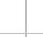
\includegraphics[max width=\textwidth]{2024_11_21_d51d653f4fe4a5bb0c33g-15}
 &  &  \\
\hline
 &  &  &  &  &  &  &  &  &  &  &  &  &  &  &  &  &  &  &  &  &  &  &  &  &  &  \\
\hline
 &  &  &  &  &  &  &  &  &  &  &  &  &  &  &  &  &  &  &  &  &  &  &  &  &  &  \\
\hline
 &  &  &  &  &  &  &  &  &  &  &  &  &  &  &  &  &  &  &  &  &  &  &  &  &  &  \\
\hline
 &  &  &  &  &  &  &  &  &  &  &  &  &  &  &  &  &  &  &  &  &  &  &  &  &  &  \\
\hline
 &  &  &  &  &  &  &  &  &  &  &  &  &  &  &  &  &  &  &  &  &  &  &  &  &  &  \\
\hline
 &  &  &  &  &  &  &  &  &  &  &  &  &  &  &  &  &  &  &  &  &  &  &  &  &  &  \\
\hline
 &  &  &  &  &  &  &  &  &  &  &  &  &  &  &  &  &  &  &  &  &  &  &  &  &  &  \\
\hline
 & . &  &  &  &  &  &  &  &  &  &  &  &  &  &  &  &  &  &  &  &  &  &  &  &  &  \\
\hline
 &  &  &  &  &  &  &  &  &  &  &  &  &  &  &  &  &  &  &  &  &  &  &  &  &  &  \\
\hline
 &  &  & 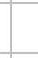
\includegraphics[max width=\textwidth]{2024_11_21_d51d653f4fe4a5bb0c33g-15(7)}
 &  &  &  &  &  &  &  &  &  &  &  &  &  &  &  &  &  &  &  &  & - &  &  \\
\hline
 &  &  & 
\includegraphics[max width=\textwidth]{2024_11_21_d51d653f4fe4a5bb0c33g-15(9)}
 &  &  &  &  &  & 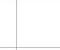
\includegraphics[max width=\textwidth]{2024_11_21_d51d653f4fe4a5bb0c33g-15(2)}
 &  &  &  &  &  &  &  &  &  &  &  & 
\includegraphics[max width=\textwidth]{2024_11_21_d51d653f4fe4a5bb0c33g-15(1)}
 & 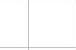
\includegraphics[max width=\textwidth]{2024_11_21_d51d653f4fe4a5bb0c33g-15(8)}
 &  &  & 
\includegraphics[max width=\textwidth]{2024_11_21_d51d653f4fe4a5bb0c33g-15(6)}
 &  \\
\hline
 &  &  &  &  &  &  &  &  &  &  &  &  &  &  &  &  &  &  &  &  &  &  &  &  &  &  \\
\hline
 &  &  &  &  &  &  &  &  & 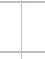
\includegraphics[max width=\textwidth]{2024_11_21_d51d653f4fe4a5bb0c33g-15(11)}
 &  &  &  &  &  &  &  & 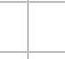
\includegraphics[max width=\textwidth]{2024_11_21_d51d653f4fe4a5bb0c33g-15(4)}
 &  &  &  & 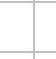
\includegraphics[max width=\textwidth]{2024_11_21_d51d653f4fe4a5bb0c33g-15(3)}
 & 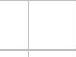
\includegraphics[max width=\textwidth]{2024_11_21_d51d653f4fe4a5bb0c33g-15(5)}
 &  & 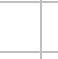
\includegraphics[max width=\textwidth]{2024_11_21_d51d653f4fe4a5bb0c33g-15(10)}
 &  &  \\
\hline
 &  &  &  &  &  &  &  &  &  &  &  &  &  &  &  &  &  &  &  &  &  &  &  &  &  &  \\
\hline
\end{tabular}
\end{center}

Odpowiedź: \(\qquad\)

\begin{center}
\begin{tabular}{|c|l|c|c|}
\hline
\multirow{2}{*}{\begin{tabular}{c}
Wypelnia \\
egzaminator \\
\end{tabular}} & Nr zadania & 26. & 27. \\
\cline { 2 - 4 }
 & Maks. liczba pkt & 2 & \(\mathbf{2}\) \\
\cline { 2 - 4 }
 & Uzyskana liczba pkt &  &  \\
\hline
\end{tabular}
\end{center}

Strona 15 z 26

\section*{Zadanie 28. (2 pkt)}
Wykaż, że dla dowolnych liczb rzeczywistych \(a\) i \(b\) prawdziwa jest nierówność

\[
3 a^{2}-2 a b+3 b^{2} \geq 0
\]

\begin{center}
\begin{tabular}{|c|c|c|c|c|c|c|c|c|c|c|c|c|c|c|c|c|c|c|c|c|c|c|}
\hline
 &  &  &  &  &  &  &  &  &  &  &  &  &  &  &  &  &  &  &  &  &  &  \\
\hline
 &  &  &  &  &  &  &  &  &  &  &  &  &  &  &  &  &  &  &  &  &  &  \\
\hline
 &  &  &  &  &  &  &  &  &  &  &  &  &  &  &  &  &  &  &  &  &  &  \\
\hline
 &  &  &  &  &  &  &  &  &  &  &  &  &  &  &  &  &  &  &  &  &  &  \\
\hline
 &  &  &  &  &  &  &  &  &  &  &  &  &  &  &  &  &  &  &  &  &  &  \\
\hline
 &  &  &  &  &  &  &  &  &  &  &  &  &  &  &  &  &  &  &  &  &  &  \\
\hline
 &  &  &  &  &  &  &  &  &  &  &  &  &  &  &  &  &  &  &  &  &  &  \\
\hline
 &  &  &  &  &  &  &  &  &  &  &  &  &  &  &  &  &  &  &  &  &  &  \\
\hline
 &  &  &  &  &  &  &  &  &  &  &  &  &  &  &  &  &  &  &  &  &  &  \\
\hline
 &  &  &  &  &  &  &  &  &  &  &  &  &  &  &  &  &  &  &  &  &  &  \\
\hline
 &  &  &  &  &  &  &  &  &  &  &  &  &  &  &  &  &  &  &  &  &  &  \\
\hline
 &  &  &  &  &  &  &  &  &  &  &  &  &  &  &  &  &  &  &  &  &  &  \\
\hline
 &  &  &  &  &  &  &  &  &  &  &  &  &  &  &  &  &  &  &  &  &  &  \\
\hline
 &  &  &  &  &  &  &  &  &  &  &  &  &  &  &  &  &  &  &  &  &  &  \\
\hline
 &  &  &  &  &  &  &  &  &  &  &  &  &  &  &  &  &  &  &  &  &  &  \\
\hline
 &  &  &  &  &  &  &  &  &  &  &  &  &  &  &  &  &  &  &  &  &  &  \\
\hline
 &  &  &  &  &  &  &  &  &  &  &  &  &  &  &  &  &  &  &  &  &  &  \\
\hline
 &  &  &  &  &  &  &  &  &  &  &  &  &  &  &  &  &  &  &  &  &  &  \\
\hline
 &  &  &  &  &  &  &  &  &  &  &  &  &  &  &  &  &  &  &  &  &  &  \\
\hline
 &  &  &  &  &  &  &  &  &  &  &  &  &  &  &  &  &  &  &  &  &  &  \\
\hline
 &  &  &  &  &  &  &  &  &  &  &  &  &  &  &  &  &  &  &  &  &  &  \\
\hline
 &  &  &  &  &  &  &  &  &  &  &  &  &  &  &  &  &  &  &  &  &  &  \\
\hline
 &  &  &  &  &  &  &  &  &  &  &  &  &  &  &  &  &  &  &  &  &  &  \\
\hline
 &  &  &  &  &  &  &  &  &  &  &  &  &  &  &  &  &  &  &  &  &  &  \\
\hline
 &  &  &  &  &  &  &  &  &  &  &  &  &  &  &  &  &  &  &  &  &  &  \\
\hline
 &  &  &  &  &  &  &  &  &  &  &  &  &  &  &  &  &  &  &  &  &  &  \\
\hline
 &  &  &  &  &  &  &  &  &  &  &  &  &  &  &  &  &  &  &  &  &  &  \\
\hline
 &  &  &  &  &  &  &  &  &  &  &  &  &  &  &  &  &  &  &  &  &  &  \\
\hline
 &  &  &  &  &  &  &  &  &  &  &  &  &  &  &  &  &  &  &  &  &  &  \\
\hline
 &  &  &  &  &  &  &  &  &  &  &  &  &  &  &  &  &  &  &  &  &  &  \\
\hline
 &  &  &  &  &  &  &  &  &  &  &  &  &  &  &  &  &  &  &  &  &  &  \\
\hline
 &  &  &  &  &  &  &  &  &  &  &  &  &  &  &  &  &  &  &  &  &  &  \\
\hline
 &  &  &  &  &  &  &  &  &  &  &  &  &  &  &  &  &  &  &  &  &  &  \\
\hline
 &  &  &  &  &  &  &  &  &  &  &  &  &  &  &  &  &  &  &  &  &  &  \\
\hline
 &  &  &  &  &  &  &  &  &  &  &  &  &  &  &  &  &  &  &  &  &  &  \\
\hline
 &  &  &  &  &  &  &  &  &  &  &  &  &  &  &  &  &  &  &  &  &  &  \\
\hline
 &  &  &  &  &  &  &  &  &  &  &  &  &  &  &  &  &  &  &  &  &  &  \\
\hline
 &  &  &  &  &  &  &  &  &  &  &  &  &  &  &  &  &  &  &  &  &  &  \\
\hline
 &  &  &  &  &  &  &  &  &  &  &  &  &  &  &  &  &  &  &  &  &  &  \\
\hline
 &  &  &  &  &  &  &  &  &  &  &  &  &  &  &  &  &  &  &  &  &  &  \\
\hline
 &  &  &  &  &  &  &  &  &  &  &  &  &  &  &  &  &  &  &  &  &  &  \\
\hline
 &  &  &  &  &  &  &  &  &  &  &  &  &  &  &  &  &  &  &  &  &  &  \\
\hline
 &  &  &  &  &  &  &  &  &  &  &  &  &  &  &  &  &  &  &  &  &  &  \\
\hline
 &  &  &  &  &  &  &  &  &  &  &  &  &  &  &  &  &  &  &  &  &  &  \\
\hline
 &  &  &  &  &  &  &  &  &  &  &  &  &  &  &  &  &  &  &  &  &  &  \\
\hline
\end{tabular}
\end{center}

\section*{Zadanie 29. (2 pkt)}
Dany jest okrąg o środku w punkcie \(S\) i promieniu \(r\). Na przedłużeniu cięciwy \(A B\) poza punkt \(B\) odłożono odcinek \(B C\) równy promieniowi danego okręgu. Przez punkty \(C\) i \(S\) poprowadzono prostą. Prosta \(C S\) przecina dany okrąg w punktach \(D\) i \(E\) (zobacz rysunek). Wykaż, że jeżeli miara kąta \(A C S\) jest równa \(\alpha\), to miara kąta \(A S D\) jest równa \(3 \alpha\).\\
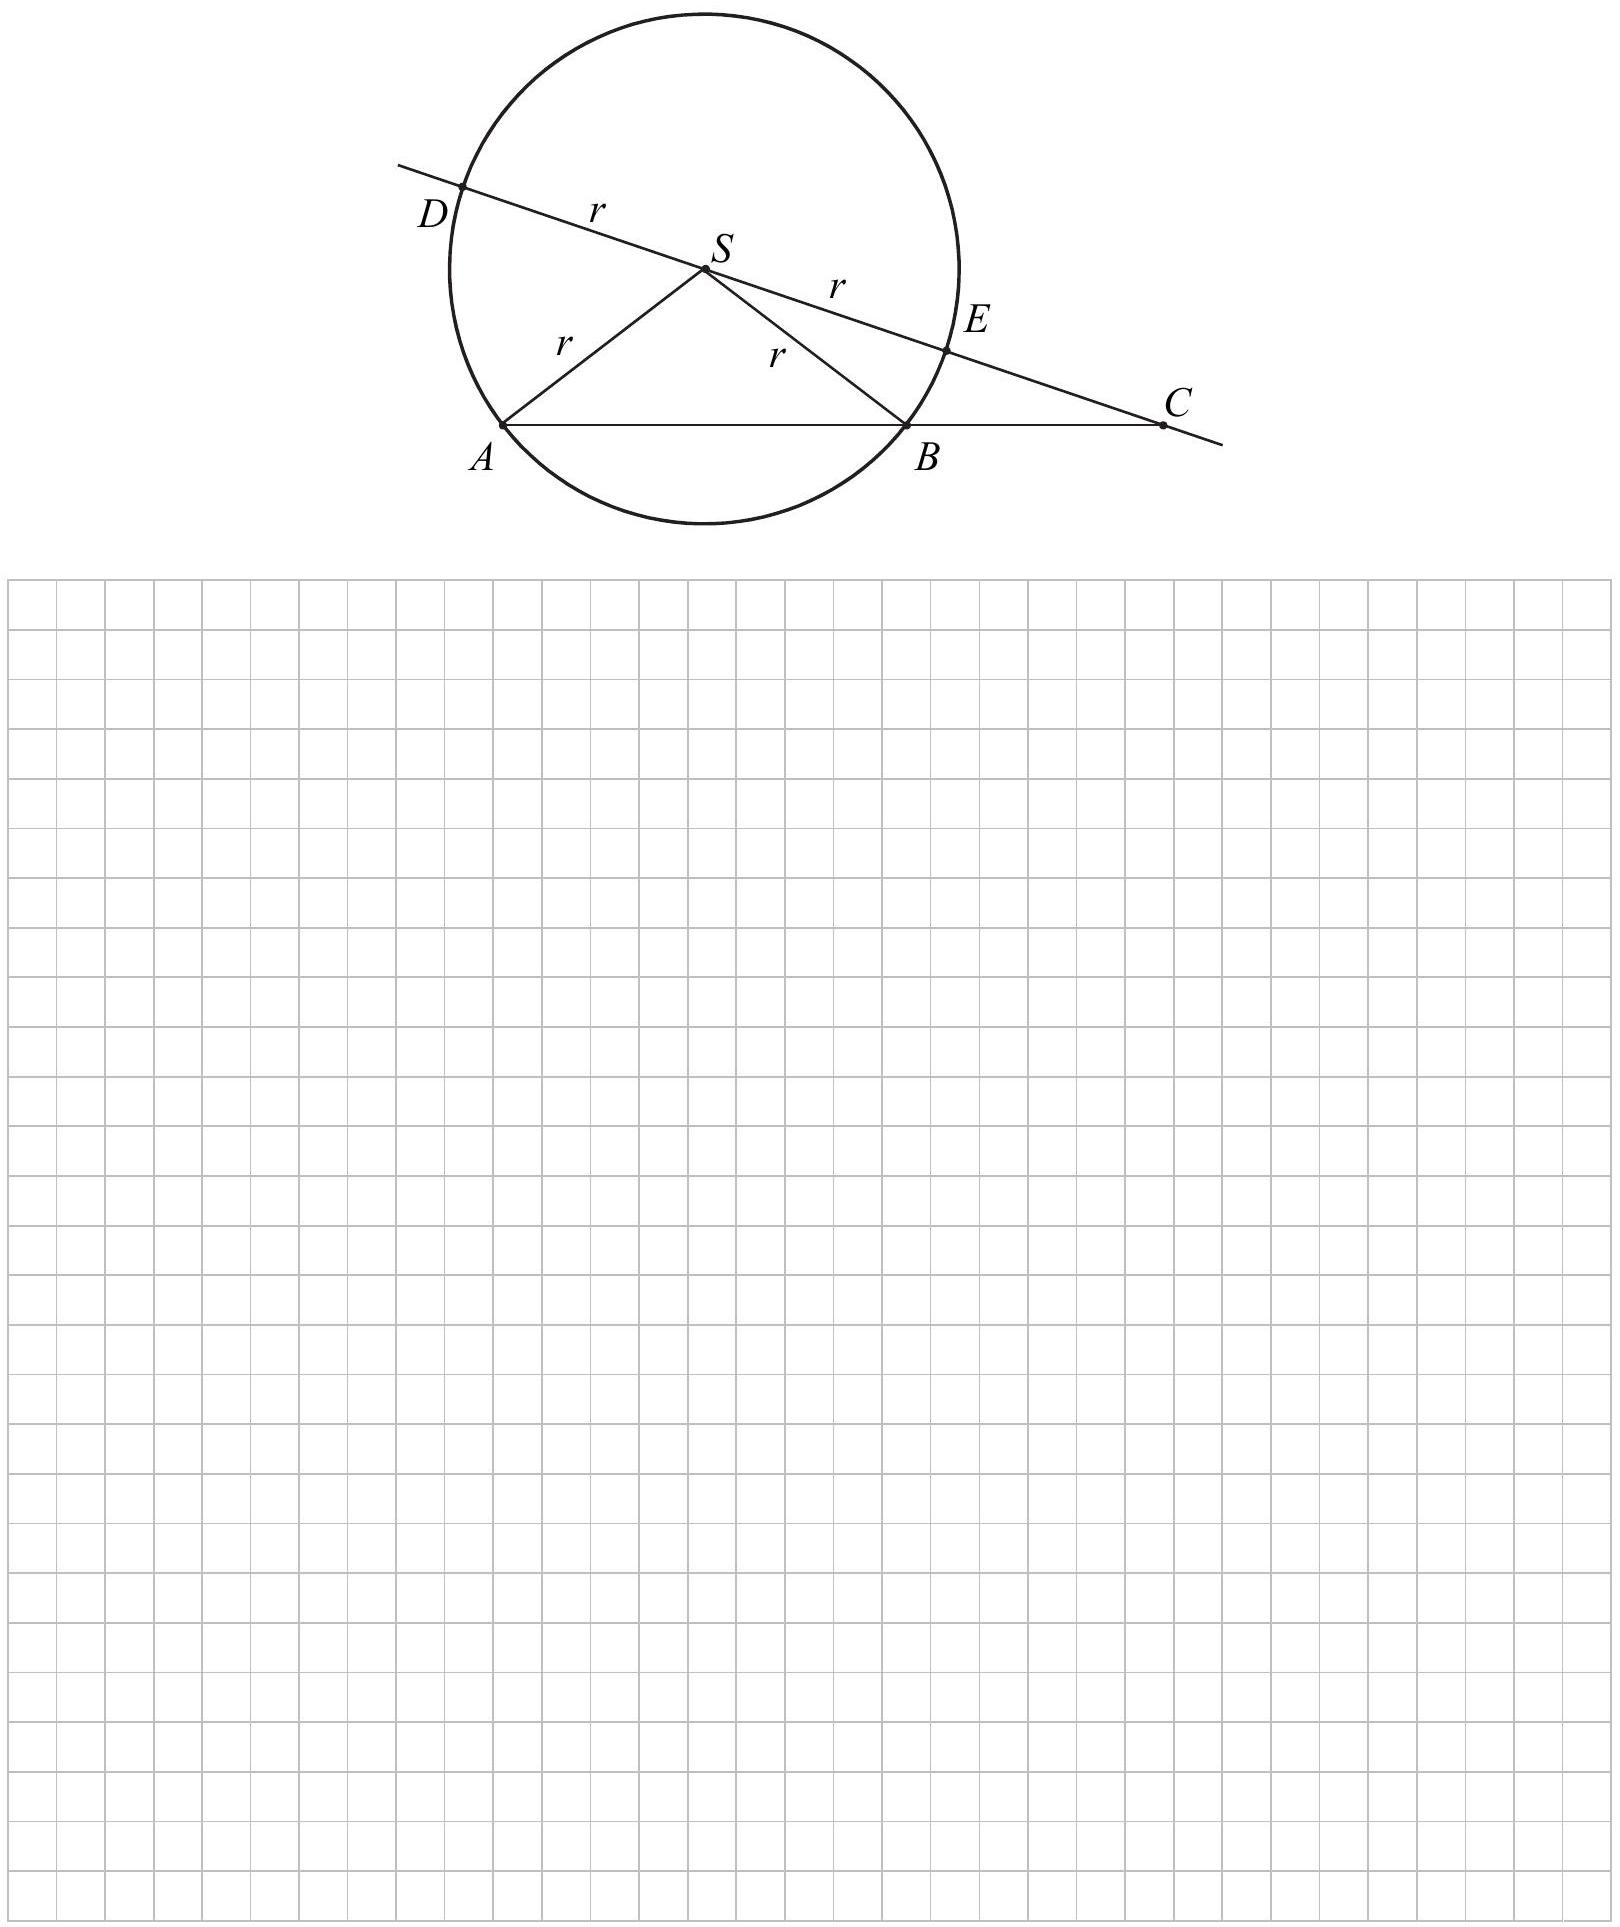
\includegraphics[max width=\textwidth, center]{2024_11_21_d51d653f4fe4a5bb0c33g-17}

\begin{center}
\begin{tabular}{|c|l|c|c|}
\hline
\multirow{2}{*}{\begin{tabular}{c}
Wypelnia \\
egzaminator \\
\end{tabular}} & Nr zadania & 28. & 29. \\
\cline { 2 - 4 }
 & Maks. liczba pkt & 2 & 2 \\
\cline { 2 - 4 }
 & Uzyskana liczba pkt &  &  \\
\hline
\end{tabular}
\end{center}

\section*{Zadanie 30. (2 pkt)}
Ze zbioru liczb \(\{1,2,3,4,5\}\) losujemy dwa razy po jednej liczbie ze zwracaniem. Oblicz prawdopodobieństwo zdarzenia \(A\) polegającego na wylosowaniu liczb, których iloczyn jest liczbą nieparzystą.\\

\includegraphics[max width=\textwidth, center]{2024_11_21_d51d653f4fe4a5bb0c33g-18}

Odpowiedź: \(\qquad\)

\section*{Zadanie 31. (2 pkt)}
W trapezie prostokątnym \(A B C D\) dłuższa podstawa \(A B\) ma długość 8 . Przekątna \(A C\) tego trapezu ma długość 4 i tworzy z krótszą podstawą trapezu kąt o mierze \(30^{\circ}\) (zobacz rysunek). Oblicz długość przekątnej \(B D\) tego trapezu.\\
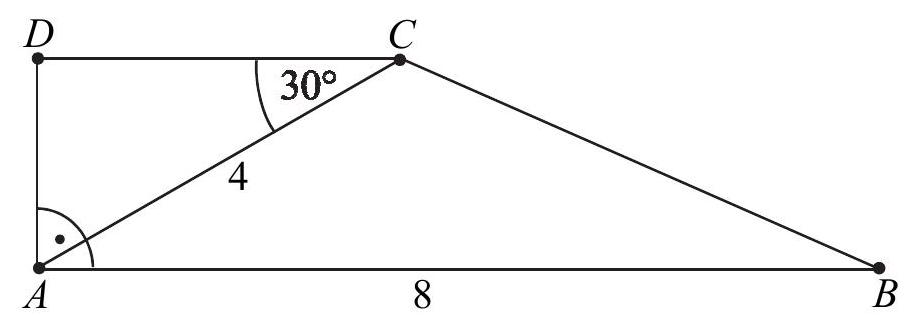
\includegraphics[max width=\textwidth, center]{2024_11_21_d51d653f4fe4a5bb0c33g-19}\\

\includegraphics[max width=\textwidth, center]{2024_11_21_d51d653f4fe4a5bb0c33g-19(1)}

Odpowiedź:

\begin{center}
\begin{tabular}{|c|l|c|c|}
\hline
\multirow{3}{*}{\begin{tabular}{c}
Wypetnia \\
egzaminator \\
\end{tabular}} & Nr zadania & 30. & 31. \\
\cline { 2 - 4 }
 & Maks. liczba pkt & \(\mathbf{2}\) & \(\mathbf{2}\) \\
\cline { 2 - 4 }
 & Uzyskana liczba pkt &  &  \\
\hline
\end{tabular}
\end{center}

Strona 19 z 26

\section*{Zadanie 32. (4 pkt)}
Cąag arytmetyczny \(\left(a_{n}\right)\) jest określony dla każdej liczby naturalnej \(n \geq 1\). Różnicą tego ciągu jest liczba \(r=-4\), a średnia arytmetyczna początkowych sześciu wyrazów tego ciągu: \(a_{1}, a_{2}, a_{3}, a_{4}, a_{5}, a_{6}\), jest równa 16.\\
a) Oblicz pierwszy wyraz tego ciągu.\\
b) Oblicz liczbę \(k\), dla której \(a_{k}=-78\).\\

\includegraphics[max width=\textwidth, center]{2024_11_21_d51d653f4fe4a5bb0c33g-20}\\

\includegraphics[max width=\textwidth, center]{2024_11_21_d51d653f4fe4a5bb0c33g-21}

Odpowiedź: \(\qquad\)

\begin{center}
\begin{tabular}{|c|l|c|}
\hline
\multirow{2}{*}{\begin{tabular}{l}
Wypelnia \\
egzaminator \\
\end{tabular}} & Nr zadania & 32. \\
\cline { 2 - 3 }
 & Maks. liczba pkt & 4 \\
\cline { 2 - 3 }
 & Uzyskana liczba pkt &  \\
\hline
\end{tabular}
\end{center}

Strona 21 z 26

\section*{Zadanie 33. (4 pkt)}
Dany jest punkt \(A=(-18,10)\). Prosta o równaniu \(y=3 x\) jest symetralną odcinka \(A B\). Wyznacz współzzędne punktu \(B\).\\

\includegraphics[max width=\textwidth, center]{2024_11_21_d51d653f4fe4a5bb0c33g-22}\\

\includegraphics[max width=\textwidth, center]{2024_11_21_d51d653f4fe4a5bb0c33g-23}

Odpowiedź: \(\qquad\)

\begin{center}
\begin{tabular}{|c|l|c|}
\hline
\multirow{3}{*}{\begin{tabular}{l}
Wypelnia \\
egzaminator \\
\end{tabular}} & Nr zadania & 33. \\
\cline { 2 - 3 }
 & Maks. liczba pkt & 4 \\
\cline { 2 - 3 }
 & Uzyskana liczba pkt &  \\
\hline
\end{tabular}
\end{center}

\section*{Zadanie 34. (5 pkt)}
Długość krawędzi podstawy ostrosłupa prawidłowego czworokątnego jest równa 6. Pole powierzchni całkowitej tego ostrosłupa jest cztery razy większe od pola jego podstawy. Kąt \(\alpha\) jest kątem nachylenia krawędzi bocznej tego ostrosłupa do płaszczyzny podstawy (zobacz rysunek). Oblicz cosinus kąta \(\alpha\).\\

\includegraphics[max width=\textwidth, center]{2024_11_21_d51d653f4fe4a5bb0c33g-24}\\

\includegraphics[max width=\textwidth, center]{2024_11_21_d51d653f4fe4a5bb0c33g-25}

Odpowiedź: \(\qquad\)

\begin{center}
\begin{tabular}{|c|l|c|}
\hline
\multirow{2}{*}{\begin{tabular}{c}
Wypelnia \\
egzaminator \\
\end{tabular}} & Nr zadania & 34. \\
\cline { 2 - 3 }
 & Maks. liczba pkt & 5 \\
\cline { 2 - 3 }
 & Uzyskana liczba pkt &  \\
\hline
\end{tabular}
\end{center}

\section*{BRUDNOPIS (nie podlega ocenie)}

\end{document}